\documentclass[oneside, 11pt]{article}

\usepackage[T1]{fontenc}
\usepackage[utf8]{inputenc}
\usepackage[dutch]{babel}

\usepackage{fouriernc}
\usepackage[detect-all, load-configurations=binary,
            separate-uncertainty=true, per-mode=symbol,
            retain-explicit-plus, range-phrase={ tot }]{siunitx}

\usepackage{setspace}
\setstretch{1.2}

\setlength{\parskip}{\smallskipamount}
\setlength{\parindent}{0pt}

\usepackage{geometry}
\geometry{marginparwidth=0.5cm, verbose, a4paper, tmargin=3cm, bmargin=3cm, lmargin=2cm, rmargin=2cm}

\usepackage{float}

\usepackage[fleqn]{amsmath}
\numberwithin{equation}{section}
\numberwithin{figure}{section}

\usepackage{graphicx}
\graphicspath{{Figures/}}
\usepackage{subfig}

\usepackage{tikz}
\usetikzlibrary{plotmarks}

\usepackage{fancyhdr}
\pagestyle{fancy}
\fancyhf{}
\rhead{\thepage}
\renewcommand{\footrulewidth}{0pt}
\renewcommand{\headrulewidth}{0pt}

\usepackage{relsize}
\usepackage{xspace}
\usepackage{url}

\newcommand{\figref}[1]{Figuur~\ref{#1}}

\newcommand{\hisparc}{\textsmaller{HiSPARC}\xspace}
\newcommand{\kascade}{\textsmaller{KASCADE}\xspace}
\newcommand{\sapphire}{\textsmaller{SAPPHiRE}\xspace}
\newcommand{\jsparc}{\textsmaller{jSparc}\xspace}
\newcommand{\hdf}{\textsmaller{HDF5}\xspace}
\newcommand{\aires}{\textsmaller{AIRES}\xspace}
\newcommand{\csv}{\textsmaller{CSV}\xspace}
\newcommand{\python}{\textsmaller{PYTHON}\xspace}
\newcommand{\corsika}{\textsmaller{CORSIKA}\xspace}
\newcommand{\labview}{\textsmaller{LabVIEW}\xspace}
\newcommand{\daq}{\textsmaller{DAQ}\xspace}
\newcommand{\adc}{\textsmaller{ADC}\xspace}
\newcommand{\adcs}{\textsmaller{ADC}s\xspace}
\newcommand{\Adcs}{A\textsmaller{DC}s\xspace}
\newcommand{\hi}{\textsc{h i}\xspace}
\newcommand{\hii}{\textsc{h ii}\xspace}
\newcommand{\mip}{\textsmaller{MIP}\xspace}
\newcommand{\hisparcii}{\textsmaller{HiSPARC II}\xspace}
\newcommand{\hisparciii}{\textsmaller{HiSPARC III}\xspace}
\newcommand{\pmt}{\textsmaller{PMT}\xspace}
\newcommand{\pmts}{\textsmaller{PMT}s\xspace}

\DeclareSIUnit{\electronvolt}{\ensuremath{\mathrm{e\!\!\:V}}}

\DeclareSIUnit{\unitsigma}{\ensuremath{\sigma}}
\DeclareSIUnit{\mip}{\textsmaller{MIP}}
\DeclareSIUnit{\adc}{\textsmaller{ADC}}

\DeclareSIUnit{\gauss}{G}
\DeclareSIUnit{\parsec}{pc}
\DeclareSIUnit{\year}{yr}


\newcolumntype{x}[1]{>{\centering\arraybackslash\hspace{0pt}}p{#1}}

\title{Air-showers, events en coïncidenties}
\author{N.G. Schultheiss}
\docdocent{1}{UA}
\version{1.0}

\begin{document}

\maketitle

\section{Inleiding}

Op de \hisparc site is RouteNet te vinden. Hierin staan modules die
als verdieping gebruikt kunnen worden. Klik bijvoorbeeld op ,,Periodieke
data verwerken'' en er verschijnt een lesbrief over het verwerken
van periodieke data. Ook dit lesmateriaal is vrij te gebruiken onder
de Creative Commons naamsvermelding / gelijk delen licentie.


\section{Events}

\begin{itemize}
    \item Een enkele detector op de grond geeft een signaal, dit wordt
    een \emph{single} genoemd. 
    \item Meerdere detectoren geven nagenoeg tegelijk een signaal, dit
    wordt een \emph{event} genoemd. 
\end{itemize}

\subsection{De nauwkeurigheid van het meten van events}

De witte led van de \hisparc unit licht op als er een event optreedt,
een simulatie is beschikbaar op
\url{http://data.hisparc.nl/media/jsparc/trigger_simulation.html} . Dit
gebeurt onder de volgende voorwaarden:

\begin{itemize}
    \item Een \textit{event} vindt plaats als het station getriggerd
    wordt. Bij een tweeplaatsstation wordt het station getriggerd als
    beide detectoren binnen \SI{1,5}{\micro\second} een signaal lager
    dan \SI{-70}{\milli\volt} afgeven. 
    \item Een vierplaatsstation wordt ook getriggerd als drie
    detectorenbinnen \SI{1,5}{\micro\second} een signaal hoger dan
    \SI{-30}{\milli\volt} afgeven. 
\end{itemize}

\begin{minipage}[t]{1\columnwidth}%

\paragraph{Opdracht 1:}

Bepaal hoe vaak het witte ledje in 1 minuut oplicht. Doe dit 5 keer
en vul de resultaten hieronder in de tabel in.

\smallskip{}


\begin{tabular}{|x{.11\textwidth}|x{.11\textwidth}|x{.11\textwidth}
                |x{.11\textwidth}|x{.11\textwidth}|x{.11\textwidth}
                |x{.11\textwidth}|}
    \cline{2-7} 
    \multicolumn{1}{c|}{} & 1 & 2 & 3 & 4 & 5 & $N_\textrm{gem}$\\
    \hline 
    $N$ &  &  &  &  &  & \tabularnewline
    \hline 
\end{tabular}%

\smallskip{}

De tabel wordt ingevuld en het gemiddelde wordt berekend.%
\end{minipage}

\bigskip{}

\begin{minipage}[t]{1\columnwidth}%

\paragraph{Opdracht 2:}

Bepaal naast het gemiddelde ook de maximale en de minimale
waarde, leg uit welke nauwkeurigheid je verwacht.

De nauwkeurigheid wordt bepaald door het verschil de maximale en gemiddelde
waarde \textit{en} het verschil van de gemiddelde en minimale waarde
te vergelijken. Bij een nette verdeling zijn deze beide waarden nagenoeg
gelijk.%
\end{minipage}

\bigskip{}


\begin{minipage}[t]{1\columnwidth}%

\paragraph{Opdracht 3:}

Bereken het gemiddelde van $N^{2}$.

\bigskip{}

\begin{tabular}{|x{.11\textwidth}|x{.11\textwidth}|x{.11\textwidth}
                |x{.11\textwidth}|x{.11\textwidth}|x{.11\textwidth}
                |x{.11\textwidth}|}
    \cline{2-7} 
    \multicolumn{1}{c|}{} & 1 & 2 & 3 & 4 & 5 & $\left(N^{2}\right)_\textrm{gem}$\\
    \hline 
    $N^{2}$ &  &  &  &  &  & \\
    \hline 
\end{tabular}


\bigskip{}

De tabel wordt ingevuld en het gemiddelde van de kwadraten wordt berekend.

\bigskip{}

De spreiding is nu te berekenen met
$\sigma=\sqrt{\left(N^{2}\right)_\textrm{gem}-\left(N_\textrm{gem}\right)^{2}}$ dit is
dus de wortel uit het gemiddelde van de kwadraten min het kwadraat van
het gemiddelde ($N_\textrm{gem}$ is al in opdracht 1 berekend).

\end{minipage}

\bigskip{}

\begin{minipage}[t]{1\columnwidth}%

\paragraph{Opdracht 4:}

Welke conclusie mag je trekken als je de waarden die je bij opdracht
2 en 3 hebt gevonden vergelijkt?

\smallskip{}

Bij een nette (Gaussische) verdeling zullen beide waarden nagenoeg
gelijk zijn. %
\end{minipage}


\subsection{Controle van de hypothese}


\subsubsection{Het signaal van een enkele detector wordt gezien als achtergrondstraling.}

\begin{minipage}[t]{1\columnwidth}%

\paragraph{Opdracht 5:}

Bereken (met een boxplot) hoe groot de kans is dat er een
tweede radioactief verval binnen \SI{1.5}{\micro\second} van de eerste
radioactief verval optreedt

\bigskip{}

Er gaat gemiddeld iedere \SI{10}{\milli\second} een deeltje door
de detector. De kans dat dit binnen \SI{1.5}{\micro\second} van een
ander deeltje gebeurd is:

\bigskip{}

$P=\frac{1,5\mu\mathrm{s}}{10\mathrm{ms}}=1,5*10^{-3}=0,15\%$%
\end{minipage}

\bigskip{}

\begin{minipage}[t]{1\columnwidth}%

\paragraph{Opdracht 6:}

Laat zien dat de met de boxplot berekende waarde nauwelijks
afwijkt van de met de Poisson-formule berekende waarde $P_{k=1}$.

\bigskip{}

$P_{k=1}=\frac{\lambda^{k}}{k!}e^{-\lambda}=\frac{\left(1,5*10^{-3}\right)}{1}e^{-\left(1,5*10^{-3}\right)}\approx1,5*10^{-3}=0,15\%$%
\end{minipage}

\bigskip{}

\begin{minipage}[t]{1\columnwidth}%

\paragraph{Opdracht 7:}

Met de kans dat er geen toevallige trigger optreed, is de
kans op een toevallige trigger ook te berekenen. (De kans op een trigger
plus de kans op geen trigger is 100\%.) Bereken deze kans.

\bigskip{}

$P_{k>0}=1-P_{k=0}=1-\frac{\left(1,5*10^{-3}\right)^{0}}{1}e^{-\left(1,5*10^{-3}\right)}=1-e^{-\left(1,5*10^{-3}\right)}\approx1,5*10^{-3}=0,15\%$
(Verdieping: Taylor reeks.)%
\end{minipage}

\bigskip{}

\begin{minipage}[t]{1\columnwidth}%

\paragraph{Opdracht 8:}

Maak de onderstaande tabel voor een station met twee detectoren
af.

\bigskip{}

\begin{tabular}{|x{.20\textwidth}|x{.07\textwidth}|x{.07\textwidth}
                |x{.07\textwidth}|x{.07\textwidth}|x{.07\textwidth}
                |x{.07\textwidth}|x{.07\textwidth}|}
    \hline 
    $T_\textrm{venster}$ {[}$\mu\mathrm{s}${]} & 1,5 & 3,0 & 7,5 & 15 & 30 & 75 & 150\tabularnewline
    \hline 
    $P_\textrm{trigger}=1-P_{k=0}$ & 0.15  & 0.30 & 0.75 & 1.5 & 3,0 & 7.2 & 14\tabularnewline
    \hline 
\end{tabular}
\end{minipage}

\bigskip{}


\begin{figure}[h]

\paragraph{Opdracht 9:}

Maak het diagram van de kans op een toevallige trigger als
functie van de duur van het triggervenster.\bigskip{}

In eerste instantie lijkt het verband nagenoeg rechtevenredig, Het
is natuurlijk zo dat er altijd een (kleine) kans zal zijn dat er geen
trigger optreedt. De lijn zal op den duur dus assymptotisch naar 100\%
gaan.
\end{figure}


\bigskip{}


\begin{minipage}[t]{1\columnwidth}%

\paragraph{Opdracht 10:}

Beredeneer hoe groot de kans op een toevallige trigger is
bij een station met 4 detectoren.

\bigskip{}

Bij vier detectoren zijn er veel combinaties mogelijk, detector 1
kan combineren met detector 2, 3 en 4. Detector 2 kan dan nog combineren
met 3 en 4. Tot slot kan detector 3 nog met detector 4 combineren.
In het totaal zijn er dus 6 verschillende combinaties met ieder een
kans van 0,15\%. De kans bij een station met vier detectoren op een
event dat door achtergrondstraling wordt veroorzaakt is: $P_{vierdetector}=6*0,15\%=0,90\%$%
\end{minipage}


\subsubsection{De gelijktijdige signalen van twee detectoren wijzen op een event.}

Van dit experimenteel onderzoek kan een meetrapport of verslag worden
gemaakt.

\bigskip{}


\begin{minipage}[t]{1\columnwidth}%

\paragraph{Opdracht 11:}

Bepaal het oppervlak in de doos in $\mathrm{cm^{2}}$. In
werkelijkheid komt dit overeen met een oppervlak in $\mathrm{m^{2}}$,
dit tweede oppervlak is te berekenen.

\bigskip{}

Deze opdracht is uitgevoerd als het aantal $\mathrm{m^{2}}$ correct
is berekend. Dus met gebruik van formule, eenheden en nauwkeurigheid.
Helaas kan er bij de kopieermachine een schaalprobleem optreden. De
kaart moet dus geijkt worden.%
\end{minipage}

\bigskip{}


\begin{minipage}[t]{1\columnwidth}%

\paragraph{Opdracht 12:}

Bereken hoeveel deeltjes nodig zijn.

\smallskip{}

\begin{tabular}{|x{.3\textwidth}|x{.1\textwidth}|x{.1\textwidth}
                |x{.1\textwidth}|x{.1\textwidth}|x{.1\textwidth}|}
    \hline 
    $\rho_\textrm{werkelijk}$ $\left[\mathrm{m^{-2}}\right]$ & 0,5 & 1 & 2 & 5 & 10 \\
    \hline 
    Aantal korreltjes in de doos &  &  &  &  & \\
    \hline 
\end{tabular}

\smallskip{}

Deze tabel is met de geijkte afmetingen in te vullen. Zonodig kan
een voorbeeldberekening worden verlangt.%
\end{minipage}

\bigskip{}


\begin{minipage}[t]{1\columnwidth}%

\paragraph{Opdracht 13:}

Bereken de massa couscous:\smallskip{}

\begin{tabular}{|x{.3\textwidth}|x{.1\textwidth}|x{.1\textwidth}
                |x{.1\textwidth}|x{.1\textwidth}|x{.1\textwidth}|}
    \hline 
    $\rho_\textrm{werkelijk}$ $\left[\mathrm{m^{-2}}\right]$ & 0,5 & 1 & 2 & 5 & 10 \\
    \hline 
    Massa couscous in de doos &  &  &  &  & \\
    \hline 
\end{tabular}

\smallskip{}


De gevoeligheid van de gebruikte weegschaal is hier van groot belang,
een ongevoelige weegschaal kan een groter aantal korreltjes nodig
hebben om de juiste massa te bepalen.%
\end{minipage}

\bigskip{}


Bij het schudden kan zowel heen en weer als op en neer geschud worden.
Let op dat de randen van de doos geen ophopingen vertonen en dat het
hele oppervlak verder redelijk gelijkmatig gevuld is. Even oefenen!

\bigskip{}


\begin{minipage}[t]{1\columnwidth}%

\paragraph{Opdracht 14:}

Voer het experiment uit een aantal keren uit en bepaal de
kans dat het station getriggerd wordt.\smallskip{}

\begin{tabular}{|>{\centering}p{2.2cm}|>{\centering}p{1cm}|>{\centering}p{1cm}
                |>{\centering}p{1cm}|>{\centering}p{1cm}|>{\centering}p{1cm}
                |>{\centering}p{1cm}|>{\centering}p{1cm}|>{\centering}p{1cm}
                |>{\centering}p{1cm}|>{\centering}p{1cm}|}
    \cline{2-11} 
    \multicolumn{1}{c|}{} & \multicolumn{5}{c|}{twee detectoren} & \multicolumn{5}{c|}{vier detectoren}\tabularnewline
    \hline 
    $\rho$ $\left[\mathrm{m^{-2}}\right]$ & 0,5 & 1 & 2 & 5 & 10 & 0,5 & 1 & 2 & 5 & 10\tabularnewline
    \hline 
    meting 1 &  &  &  &  &  &  &  &  &  & \tabularnewline
    \hline 
    meting 2 &  &  &  &  &  &  &  &  &  & \tabularnewline
    \hline 
    meting 3 &  &  &  &  &  &  &  &  &  & \tabularnewline
    \hline 
    meting 4 &  &  &  &  &  &  &  &  &  & \tabularnewline
    \hline 
    meting 5 &  &  &  &  &  &  &  &  &  & \tabularnewline
    \hline 
    meting 6 &  &  &  &  &  &  &  &  &  & \tabularnewline
    \hline 
    meting 7 &  &  &  &  &  &  &  &  &  & \tabularnewline
    \hline 
    meting 8 &  &  &  &  &  &  &  &  &  & \tabularnewline
    \hline 
    meting 9 &  &  &  &  &  &  &  &  &  & \tabularnewline
    \hline 
    meting 10 &  &  &  &  &  &  &  &  &  & \tabularnewline
    \hline 
    kans op trigger &  &  &  &  &  &  &  &  &  & \tabularnewline
    \hline 
\end{tabular}

\smallskip{}


De kans op een trigger bij 10 steekproeven is 10\%, 20\%, 30\% etc.%
\end{minipage}

\bigskip{}


\begin{figure}[h]
    \paragraph{Opdracht 15:}

    Maak het diagram voor een station met twee en een station
    met vier detectoren.\bigskip{}

    
\begin{tikzpicture}
        [gridlines/.style={color=gray,very thin}]
        \draw [gridlines, step=.5cm] (0,0) grid (\textwidth,8cm);
    \end{tikzpicture}

    \smallskip{}

    Uiteraard zijn de assen van grootheden en eenheden voorzien. De waarden
    verspringen in stappen van 10\%. Dit heeft gevolgen voor de nauwkeurigheid
    ($\pm10\%$ ?). 

    \bigskip{}

    \caption{Het diagram van de triggerkans als functie van de deeltjesdichtheid $\rho$.}
\end{figure}


\bigskip{}


\begin{minipage}[t]{1\columnwidth}

\paragraph{Opdracht 16:}

Ook bij coïncidenties kan een triggervenster worden gebruikt.
Dit venster hangt af van de afstand tussen de stations en de lichtsnelheid.
De air-shower geeft het grootste tijdverschil als deze horizontaal
door de opstelling beweegt. Een dergelijke air-shower wordt gegenereerd
door een primair kosmisch deeltje met een extreem grote energie. In
de praktijk komen deze air-showers zelden voor.

Bereken de grootte van het triggervenster in de volgende gevallen:

$t=\frac{s}{c}$

\bigskip{}


\begin{tabular}{|c|>{\centering}p{2cm}|>{\centering}p{2cm}|>{\centering}p{2cm}|>{\centering}p{2cm}|}
    \hline 
    Afstand tussen de stations {[}m{]} & 100 & 200 & 500 & 1000\tabularnewline
    \hline 
    Duur van het triggervenster {[}ns{]} & $3,33*10^{2}$ & $6,67*10^{2}$ & $1,67*10^{3}$ & $3,33*10^{3}$\tabularnewline
    \hline 
\end{tabular}
\end{minipage}

\bigskip{}
\begin{minipage}[t]{1\columnwidth}%

\paragraph{Opdracht 17:}

Het bepalen van de bin-breedte -de afstand tussen de bin waarden-
verdient enige aandacht. Als de frequentie van verschilwaarden laag
is, is het niet handig om een kleine bin-breedte te nemen. De frequentie
hangt namelijk af van de bin-breedte. Een kleine bin-breedte geeft
een lage frequentie, maar een grote nauwkeurigheid in de tijd. Een
grote bin-breedte geeft een hoge frequentie maar een kleine nauwkeurigheid
in de tijd.

Bedenk een methode om de bin-breedte handig te kiezen als
het totale aantal verschiltijden (coïncidenties) (N) en de minimale
($t_\textrm{min}$) en maximale ($t_\textrm{max}$) bin-waarde bekend zijn.

Indien er $N$ coincidenties zijn vullen deze alle bins. Als het oppervlak
eerlijk verdeeld wordt, geldt $N=f_\textrm{gem}*n_\textrm{bin}$ waarin $n_\textrm{bin}$
het aantal bins of staven in het diagram is. Als de resolutie langs
de $f$-as en de $bin$-as gelijk is, geldt $2f_\textrm{gem}\approx f_\textrm{max}=n_\textrm{bin}$
of $2N\approx\left(n_\textrm{bin}\right)^{2}\Rightarrow n_\textrm{bin}\approx\sqrt{2N}$.
De bin-breedte wordt dan ongeveer $\frac{t_\textrm{max}-t_\textrm{min}}{\sqrt{2N}}$.
Let wel op dat de frequentie van de eerste en laatste bins voldoende
is. %
\end{minipage}

\bigskip{}

\begin{figure}[p]
    \centering
    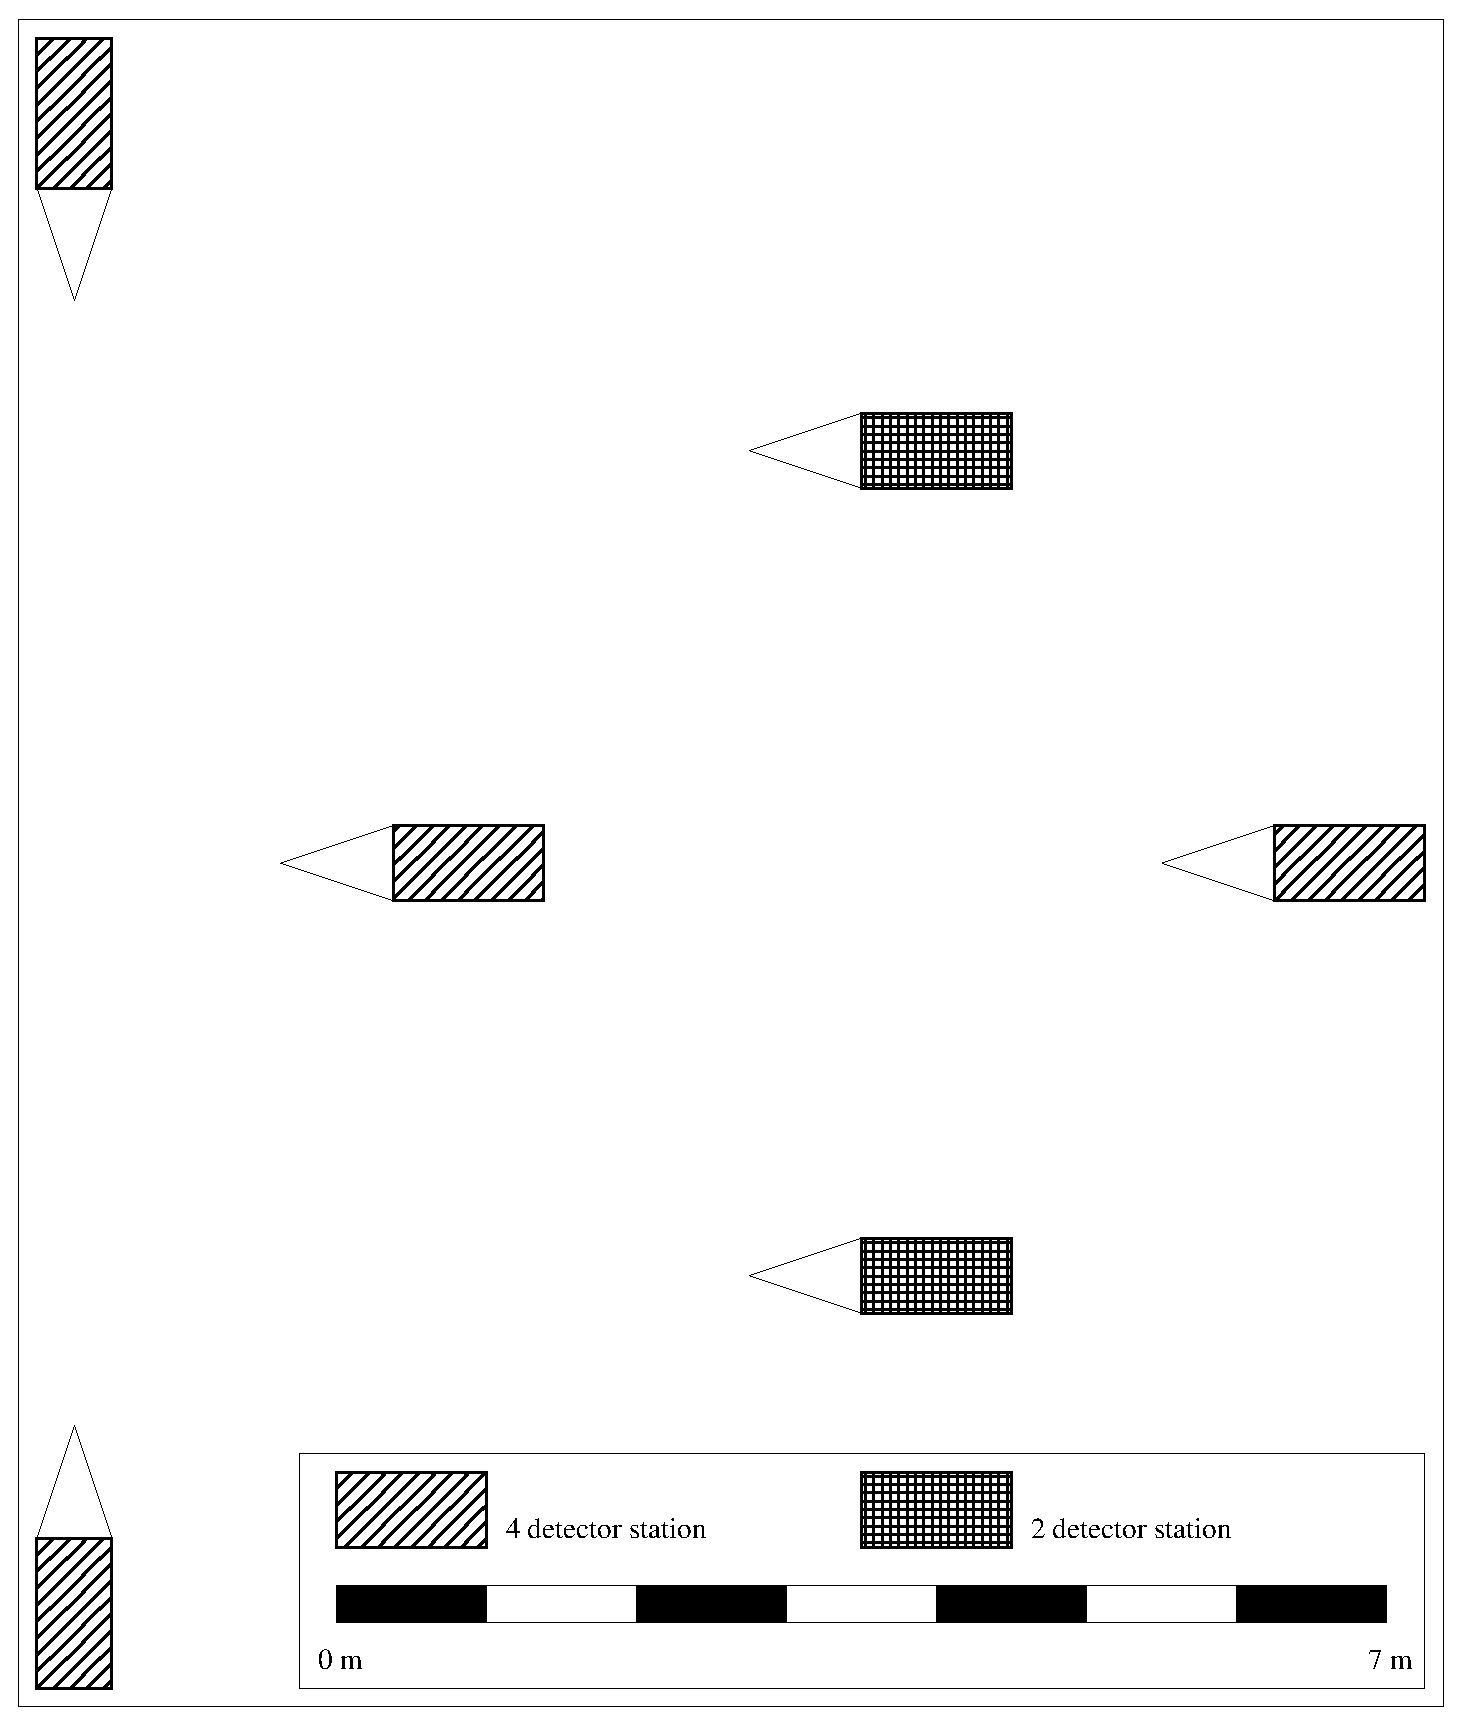
\includegraphics[width=15.833cm]{Figures/station}
    \caption{\label{fig:Meetstations}Meetstations}
\end{figure}

\end{document}
